\documentclass{standalone}
% font set
\usepackage{ctex}
\usepackage{fontspec}
\usepackage[T1]{fontenc}
\usepackage[sc]{mathpazo}
\usepackage{anyfontsize}
\setmainfont{Source Serif 4}
\setsansfont{Source Sans 3}
\setmonofont{Menlo}
\setCJKmainfont[BoldFont=黑体-简 中等,ItalicFont=楷体-简 常规体]{宋体-简 常规体}

% colors
\usepackage[dvipsnames]{xcolor}
\definecolor{pku-red}{RGB}{139,0,18}
\usepackage{colortbl}
\newcommand{\light}[1]{\textcolor{Orchid}{#1}}
\newcommand{\contrastlight}[1]{\textcolor{TealBlue}{#1}}

% plots
\usepackage{tikz}
\usepackage{tikz-cd}
\usetikzlibrary{arrows}
\usetikzlibrary{arrows.meta,positioning,calc,3d}
\usepackage{tikz-3dplot}
\usepackage{pgfplots}
\pgfplotsset{compat=newest}

% math package
\let\Bbbk\relax
\usepackage{amsmath}
\usepackage{mathrsfs}
\usepackage{amssymb}
\usepackage{amsfonts}
\usepackage{stmaryrd}
\usepackage{latexsym}
\usepackage{extarrows}
\SetSymbolFont{stmry}{bold}{U}{stmry}{m}{n}


% math notations
\newcommand{\LHS}{\mathrm{LHS}}
\newcommand{\RHS}{\mathrm{RHS}}
\newcommand{\Z}{\mathbb{Z}}
\newcommand{\N}{\mathbb{N}}
\newcommand{\R}{\mathbb{R}}
\newcommand{\Q}{\mathbb{Q}}
\newcommand{\C}{\mathbb{C}}
\newcommand{\E}{\mathbb{E}}
\renewcommand{\O}{\mathcal{O}}
\newcommand{\id}{\mathrm{id}}
\DeclareMathOperator*{\Span}{Span}
\DeclareMathOperator*{\im}{Im}
\DeclareMathOperator*{\rank}{rank}
\DeclareMathOperator*{\card}{card}
\DeclareMathOperator*{\grad}{grad}
\DeclareMathOperator*{\argmax}{argmax}
\DeclareMathOperator*{\epi}{epi}
\DeclareMathOperator*{\maximize}{maximize}
\DeclareMathOperator*{\minimize}{minimize}
\renewcommand{\d}{\mathrm{d}}
\newcommand{\Pow}{\mathcal{P}}
\newcommand{\cov}{\mathsf{Cov}}
\newcommand{\var}{\mathsf{Var}}
\newcommand{\Nor}{\mathcal{N}}
\newcommand{\U}{\mathcal{U}}
\renewcommand{\t}{\mathsf{T}}
\newcommand{\T}{\top}
\newcommand{\F}{\bot}
\newcommand{\norm}[1]{\left\|#1\right\|}
\newcommand{\inner}[2]{\left\langle{#1},{#2}\right\rangle}
\newcommand{\e}{\mathrm{e}}
\newcommand{\const}{\mathrm{const}}
\newcommand{\scB}{\mathscr{B}}
\newcommand{\scF}{\mathscr{F}}
\newcommand{\G}{\mathscr{G}}
\newcommand{\Exp}{\mathsf{Exp}}
\newcommand{\DExp}{\mathsf{DExp}}
\newcommand{\Lap}{\mathsf{Lap}}
\newcommand{\calP}{\mathcal P}
\newcommand{\calS}{\mathcal S}
\newcommand{\calF}{\mathcal F}
\newcommand{\calM}{\mathcal M}
\newcommand{\KL}{\mathrm{KL}}
\newcommand{\ReLU}{\mathsf{ReLU}}
\newcommand{\val}{\mathsf{val}}

\newcommand{\drawGrid}{
    \draw[line width=2] (-0.8,0) -- (0.8,0);
    \draw[line width=2] (-0.8,0.5) -- (0.8,0.5);
    \draw[line width=2] (-0.8,-0.5) -- (0.8,-0.5);
    \draw[line width=2] (0,-0.8) -- (0,0.8);
    \draw[line width=2] (-0.5,-0.8) -- (-0.5,0.8);
    \draw[line width=2] (0.5,-0.8) -- (0.5,0.8);
}

\newcommand{\drawW}[2]{\draw[fill=white, draw=black, line width=1] (#1*0.5, #2*0.5) circle(0.15);}
\newcommand{\drawB}[2]{\draw[fill=black, draw=black, line width=1] (#1*0.5, #2*0.5) circle(0.15);}

\newcommand{\randDistOne}{%
     \fill[TealBlue,opacity=0.6] (0,0) rectangle ++(0.9,4);
        \fill[TealBlue,opacity=0.6] (1,0) rectangle ++(0.9,0.2);
        \fill[TealBlue,opacity=0.6] (2,0) rectangle ++(0.9,3.6);
        \fill[TealBlue,opacity=0.6] (3,0) rectangle ++(0.9,5);
        \fill[TealBlue,opacity=0.6] (4,0) rectangle ++(0.9,3.8);
        \fill[TealBlue,opacity=0.6] (5,0) rectangle ++(0.9,0.6);
}

\newcommand{\randDistTwo}{%
    \fill[TealBlue,opacity=0.6] (0,0) rectangle ++(0.9,2.3);
    \fill[TealBlue,opacity=0.6] (1,0) rectangle ++(0.9,4.1);
    \fill[TealBlue,opacity=0.6] (2,0) rectangle ++(0.9,1.7);
    \fill[TealBlue,opacity=0.6] (3,0) rectangle ++(0.9,3.9);
    \fill[TealBlue,opacity=0.6] (4,0) rectangle ++(0.9,2.8);
    \fill[TealBlue,opacity=0.6] (5,0) rectangle ++(0.9,0.5);
}

\newcommand{\randDistThree}{%
    \fill[TealBlue,opacity=0.6] (0,0) rectangle ++(0.9,3.2);
    \fill[TealBlue,opacity=0.6] (1,0) rectangle ++(0.9,1.5);
    \fill[TealBlue,opacity=0.6] (2,0) rectangle ++(0.9,4.8);
    \fill[TealBlue,opacity=0.6] (3,0) rectangle ++(0.9,2.7);
    \fill[TealBlue,opacity=0.6] (4,0) rectangle ++(0.9,4.3);
    \fill[TealBlue,opacity=0.6] (5,0) rectangle ++(0.9,0.9);
}
\begin{document}

\begin{tikzpicture}[>=Latex,font=\LARGE]
\begin{scope}
\node[label=above:$s_1$] (s1) at (0,0) {
\begin{tikzpicture}
    \drawGrid;
\end{tikzpicture}
};
\node[below=0.8 of s1] (f1) {
$f_\theta$
};
\node[below left=0.8 of f1,TealBlue,fill=TealBlue!40,circle,draw=TealBlue,very thick] (p1) {$p_1$};
\node[below right=0.8 of f1,Orchid,fill=Orchid!40,circle,draw=Orchid,very thick] (v1) {$v_1$};
\node[below=0.1 of p1] (p1approx) {\rotatebox[origin=c]{-90}{$\approx$}};
\node[below=0.1 of v1] (v1approx) {\rotatebox[origin=c]{-90}{$\approx$}};
\node[below=0.1 of p1approx, label=below:$\pi_1$] (pi1) {

\begin{tikzpicture}[scale=0.2]
    \randDistOne;
\end{tikzpicture}
};
\draw[->,line width=2] (s1) -- (f1);
\draw[dash pattern=on 0pt off 2\pgflinewidth,line cap=round,line width=2] (f1) -- (p1);
\draw[dash pattern=on 0pt off 2\pgflinewidth,line cap=round,line width=2] (f1) -- (v1);
\end{scope}

\begin{scope}
\node[label=above:$s_2$] (s2) at (5,0) {
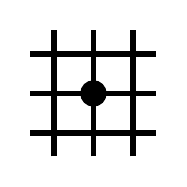
\begin{tikzpicture}
    \drawGrid;
    \drawB{0}{0};
\end{tikzpicture}
};
\node[below=0.8 of s2] (f2) {
$f_\theta$
};
\node[below left=0.8 of f2,TealBlue,fill=TealBlue!40,circle,draw=TealBlue,very thick] (p2) {$p_2$};
\node[below right=0.8 of f2,Orchid,fill=Orchid!40,circle,draw=Orchid,very thick] (v2) {$v_2$};
\node[below=0.1 of p2] (p2approx) {\rotatebox[origin=c]{-90}{$\approx$}};
\node[below=0.1 of v2] (v2approx) {\rotatebox[origin=c]{-90}{$\approx$}};
\node[below=0.1 of p2approx, label=below:$\pi_2$] (pi2) {

\begin{tikzpicture}[scale=0.2]
    \randDistTwo;
\end{tikzpicture}
};
\draw[->,line width=2] (s2) -- (f2);
\draw[dash pattern=on 0pt off 2\pgflinewidth,line cap=round,line width=2] (f2) -- (p2);
\draw[dash pattern=on 0pt off 2\pgflinewidth,line cap=round,line width=2] (f2) -- (v2);
\end{scope}

\begin{scope}
\node[label=above:$s_3$] (s3) at (10,0) {
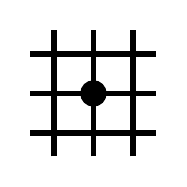
\begin{tikzpicture}
    \drawGrid;
    \drawB{0}{0};
\end{tikzpicture}
};
\node[below=0.8 of s3] (f3) {
$f_\theta$
};
\node[below left=0.8 of f3,TealBlue,fill=TealBlue!40,circle,draw=TealBlue,very thick] (p3) {$p_3$};
\node[below right=0.8 of f3,Orchid,fill=Orchid!40,circle,draw=Orchid,very thick] (v3) {$v_3$};
\node[below=0.1 of p3] (p3approx) {\rotatebox[origin=c]{-90}{$\approx$}};
\node[below=0.1 of v3] (v3approx) {\rotatebox[origin=c]{-90}{$\approx$}};
\node[below=0.1 of p3approx, label=below:$\pi_3$] (pi3) {

\begin{tikzpicture}[scale=0.2]
    \randDistThree;
\end{tikzpicture}
};
\draw[->,line width=2] (s3) -- (f3);
\draw[dash pattern=on 0pt off 2\pgflinewidth,line cap=round,line width=2] (f3) -- (p3);
\draw[dash pattern=on 0pt off 2\pgflinewidth,line cap=round,line width=2] (f3) -- (v3);
\end{scope}

\node[Orchid] (z) at (15,-8) {$z$};
\draw[->,line width=4,rounded corners=0.5cm] (z) -| (v3approx);
\draw[->,line width=4,rounded corners=0.5cm] (z) -| (v2approx);
\draw[->,line width=4,rounded corners=0.5cm] (z) -| (v1approx);

\end{tikzpicture}
\end{document}
